\begin{figure}
\centering
\pgfplotsset{compat=1.17}
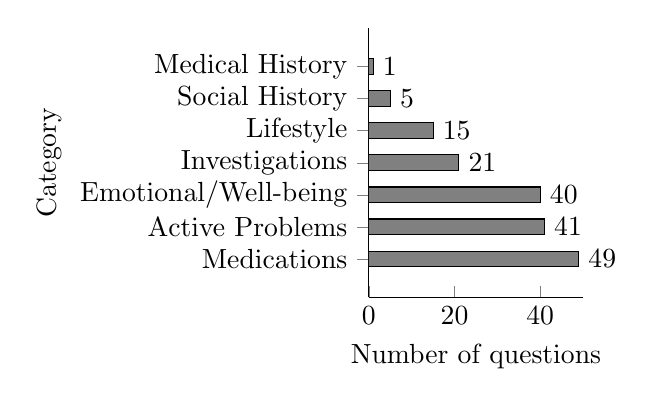
\begin{tikzpicture}
    \begin{axis}[
        xbar,
        width=4.3cm,
        height=5cm,
        bar width=0.2cm,
        nodes near coords,
        nodes near coords align={horizontal},
        xlabel={Number of questions},
        ylabel={Category},
        symbolic y coords={Medications, Active Problems, Emotional/Well-being, Investigations, Lifestyle, Social History, Medical History},
        ytick=data,
        xmin=0,
        xmax=50,
        enlarge y limits=0.2,
        axis x line*=bottom,
        axis y line*=left,
        ]
        \addplot [fill=gray, draw=black] coordinates {
            (49,Medications)
            (5,Social History)
            (41,Active Problems)
            (21,Investigations)
            (40,Emotional/Well-being)
            (15,Lifestyle)
            (1,Medical History)
        };
        % \draw[blue,dashed] ({axis cs:18.92,0}|-{rel axis cs:0,0}) -- ({axis cs:18.92,0}|-{rel axis cs:0,1}) node [pos=0.9, right] {STD = 18.92\%};
        % \draw[red,solid] ({axis cs:24.57,0}|-{rel axis cs:0,0}) -- ({axis cs:24.57,0}|-{rel axis cs:0,1}) node [pos=0.7, right] {Avg (24.57\%)};
    \end{axis}
\end{tikzpicture}
\caption{Number of questions asked in each category during the mock SRMs.}
\label{fig:question-categories}
\end{figure}